\documentclass[letterpaper, 12 pt, conference]{ieeeconf}  
\IEEEoverridecommandlockouts      
\overrideIEEEmargins
\usepackage{graphicx} % for pdf, bitmapped graphics files
\usepackage{bm}
\newcommand{\uvec}[1]{\boldsymbol{\hat{\textbf{#1}}}}

\usepackage[utf8]{inputenc}
\usepackage{vmargin}

\usepackage{mathtools}
\usepackage{amsmath} 
\usepackage{graphicx}
\usepackage{graphics}
\usepackage{float}
\usepackage{blindtext}
\usepackage{listings}
\usepackage{xcolor}
\usepackage[spanish]{babel}
\usepackage{subfig}
\usepackage{amsmath}
\usepackage{verbatim}
\graphicspath{ {images/} }
\date{}
\setpapersize{A4}
\setmargins{2.5cm}       % margen izquierdo
{1.5cm}                        % margen superior
{16.5cm}                      % anchura del texto
{23.42cm}                    % altura del texto
{10pt}                           % altura de los encabezados
{1cm}                           % espacio entre el texto y los encabezados
{0pt}                             % altura del pie de página
{2cm}                           % espacio entre el texto y el pie de página



%-------COLORES PARA CODIGO ------------------------
\lstdefinestyle{customc}{
  belowcaptionskip=1\baselineskip,
  breaklines=true,
  frame=L,
  xleftmargin=\parindent,
  language=JavaScript,
   basicstyle=\footnotesize\ttfamily,
  showstringspaces=false,
  basicstyle=\footnotesize\ttfamily,
  keywordstyle=\bfseries\color{green!40!black},
  commentstyle=\itshape\color{purple!40!black},
  identifierstyle=\color{blue},
  stringstyle=\color{orange},
  frame=single,	  
  numbers=left,
   numberstyle=\footnotesize,
}

\lstdefinestyle{customasm}{
  belowcaptionskip=1\baselineskip,
  frame=L,
  xleftmargin=\parindent,
  language=JavaScript,
  basicstyle=\footnotesize\ttfamily,
  commentstyle=\itshape\color{purple!40!black},
}

\lstset{escapechar=@,style=customc}

\title{\LARGE \bf
ECUACIÓN DE ONDA
}
\author{Andy G. Ñaca Rodriguez}
\begin{document}
\maketitle
\thispagestyle{empty}
\pagestyle{empty}
\begin{comment}
\begin{figure}[H]
    \centering
    \includegraphics[width=0.7\textwidth]{}
    \caption{}
\end{figure}
\begin{lstlisting}[language=Python,caption=]
\end{lstlisting}
\end{comment}
\begin{abstract}
En este documento se analizara la importancia y comportamiento de la ecuación de onda con distintas condiciones iniciales, incluso alterando la función inicial, obteniendo resultados interesantes. Además se podrá verificar la influencia de cumplir o no la condición de estabilidad, con los resultados obtenidos, algunos muy irregulares e incorrectos. Asimismo, se apreciara como es que la ecuación de onda a pesar de todas las deformaciones en cada iteración, llega a su estado inicial para repetir el mismo ciclo infinitamente.
\end{abstract}
\section{Introducción}
El movimiento ondulatorio esta presente en todos lados, como la luz del sol, que es una onda electromagnética que viaja a lo largo del espacio y llega a la tierra, esta onda caliente y puede entenderse que esta transmite energía. Otro ejemplo es lo onda que transmitimos al hablar, ya que hay una vibración de moléculas, que llega a nuestro oído. Es por esto que en esta practica estudiaremos este tipo de ecuación tomando en cuenta el valor que se cumpla la ecuación: $v*h/k\leq 1$ , ya que como veremos mas adelante determinara la estabilidad en nuestro problema. Además se vera como afecta la velocidad de la onda, ya que a mas velocidad se obtendrán mas ondas.
\section{Función de la ecuación de onda}
Para realizar esta parte definimos la siguiente función en Python, para que esta funcione igual que en Octave, debemos tener cuidado con los índices y los valores de i en el primer for, se debe iniciar con el mismo valor de i osea 2, pero la posición en nuestra matriz empieza desde 1, es por esto que restamos 1 a i al acceder a la matriz, empezar desde 1 en el bucle alteraría los valores que enviemos a la función ''fval()'', obteniendo resultados incorrectos.\\
Fuera de esta observación importante, el procedimiento sera el mismo, es decir calculamos manualmente las dos primeras columnas y a partir de estas las siguientes, con los dos 2 for.
\begin{lstlisting}[language=Python,caption=Ecuación de onda]
def onda(a,b,v,h,k):
    global x,y,U
    x=np.arange(0,a+h,h)
    y=np.arange(0,b+k,k)
    n=len(x)
    m=len(y)
    r=v*k/h
    r1=r**2;
    r2=r**2/2;
    s1=1-r**2;
    s2=2*(1-r**2);
    U=np.zeros((n,m));
    for i in range(2,n):
        U[i-1,0]=feval('f',h*(i-1));
        U[i-1,1]=s1*feval('f',h*(i-1))+k*feval('g',h*(i-1))+r2*(feval('f',h*i)+feval('f',h*(i-2)));
    for j in range(1,m-1):
        for i in range(1,n-1):
            U[i,j+1]= s2*U[i,j]+r1*(U[i-1,j]+U[i+1,j])-U[i,j-1];
    graficar(U,'Onda')
\end{lstlisting}
\section{Problema I}
Primero mostraremos el resultado original, con los valores indicados en el problema es decir con $h=0.05, k=0.01$ y $v=2$. Como podremos ver el resultado es correcto ya que se forman las ondas a lo largo de todo el gráfico.
\begin{figure}[H]
    \centering
    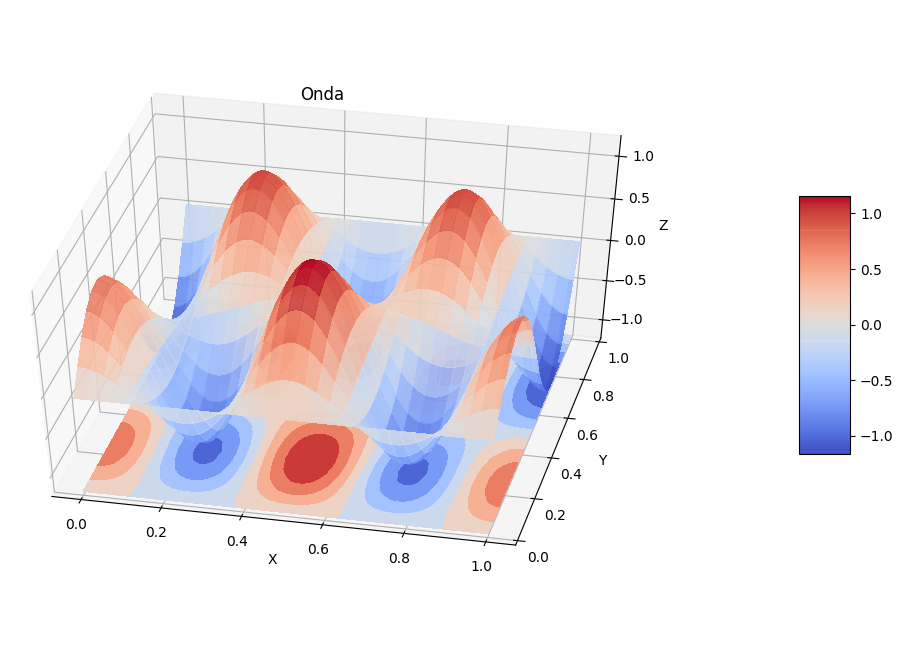
\includegraphics[width=0.5\textwidth]{h 0.05 k 0.01.png}
    \caption{Valores iniciales del problema}
\end{figure}
\subsection{ Analice el mismo problema, cambiando h y k y verifique sus resultados}
Para este problema se cambiaron los valores para tener una velocidad mayor de las que hicimos en clase, como podremos ver en la imagen esto afecta la cantidad de ondas que se generan.
\begin{figure}[H]
    \centering
    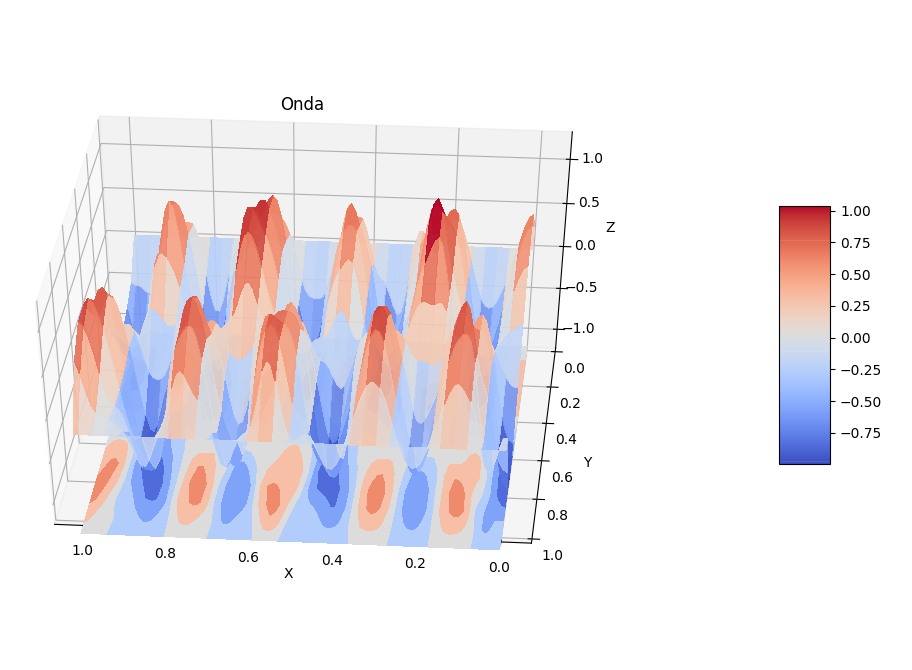
\includegraphics[width=0.5\textwidth]{v 5.png}
    \caption{Valores con v=5,h=0.09,k=0.01}
\end{figure}
\subsection{Verifique que si no cumple r $\leq$ 1, como se verán los resultados ?}
Al no cumplir la condición de que r sea menor a o igual 1, no se genera una estabilidad y los valores salen del rango permitido o lógico, como podremos ver en el eje z, estos superan el valor de 2, cuando sabemos que el rango de la función de onda es entre 1 y -1. Obteniendo así diseños que no se pueden traficar correctamente.
\begin{figure}[H]
    \centering
    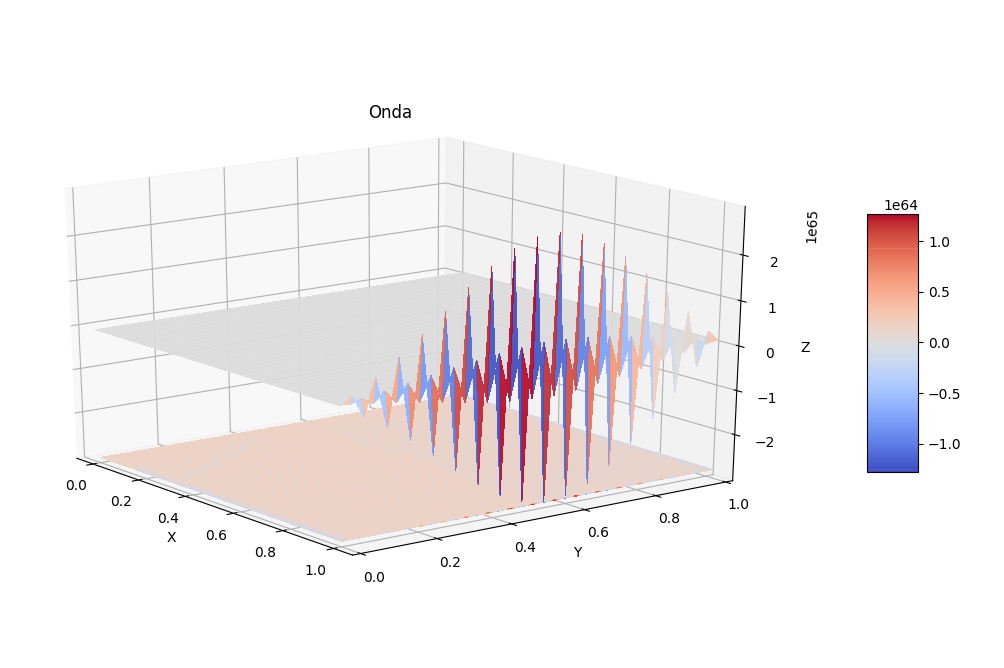
\includegraphics[width=0.5\textwidth]{r mayor 1.png}
    \caption{Valores con r>1}
\end{figure}
\section{Problema Desafió}
\subsection{Use a = 1, b = 1, v = 1, g(x) = 0}
Para este problema usaremos una función de forma triangular, gracias a la estructura de su función, las condiciones y rangos, esto se podrá evidenciar en la primera iteración del gráfico siguiente. Lo que pasara después es que esta ecuación se ira expandiendo hasta llegar a invertirse y luego volver a su condición inicial, repitiendo así este ciclo sin alteraciones debido a que no se presenta otra forma que lo altere.
\begin{figure}[H]
    \centering
    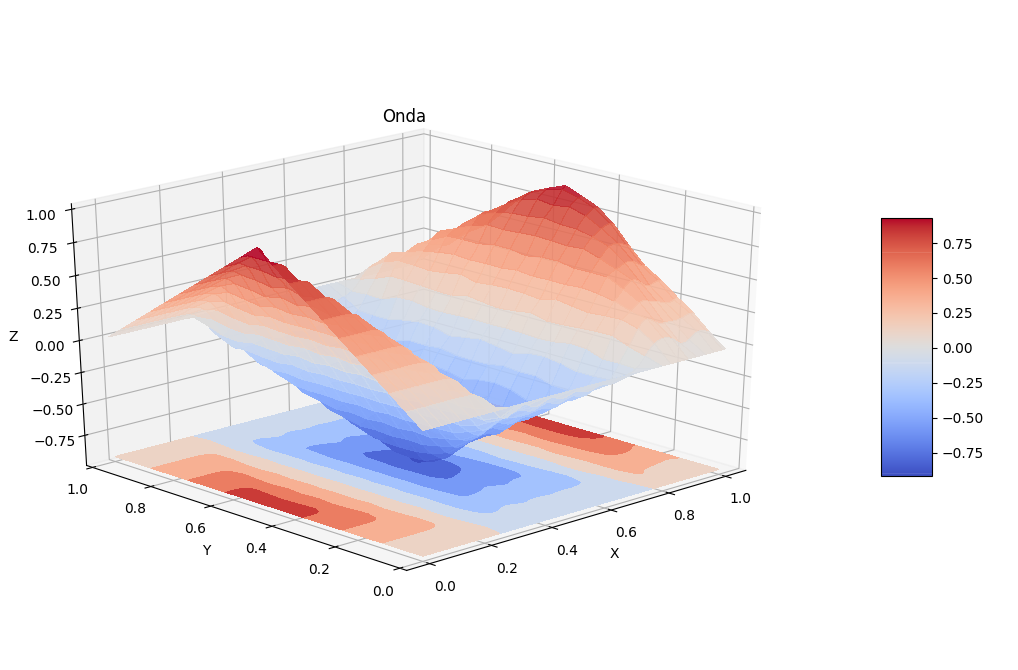
\includegraphics[width=0.5\textwidth]{desafio.png}
    \caption{Desarrollo del problema completo}
\end{figure}
\subsection{Evolución}
Para poder apreciar el cambio que tiene la función mencionada anteriormente, solo se mostrara una función de 2 dimensiones. Como veremos en cada iteración se deformara la figura inicial, pero de manera simétrica. Llega a alterarse tanto que no existe una iteración en la que la imagen sea recta, lo curioso es que a pesar de todas esas deformaciones y alteraciones llega al mismo punto inicial, esto podrá apreciarse mejor en la animación.
\begin{figure}[H]
    \centering
    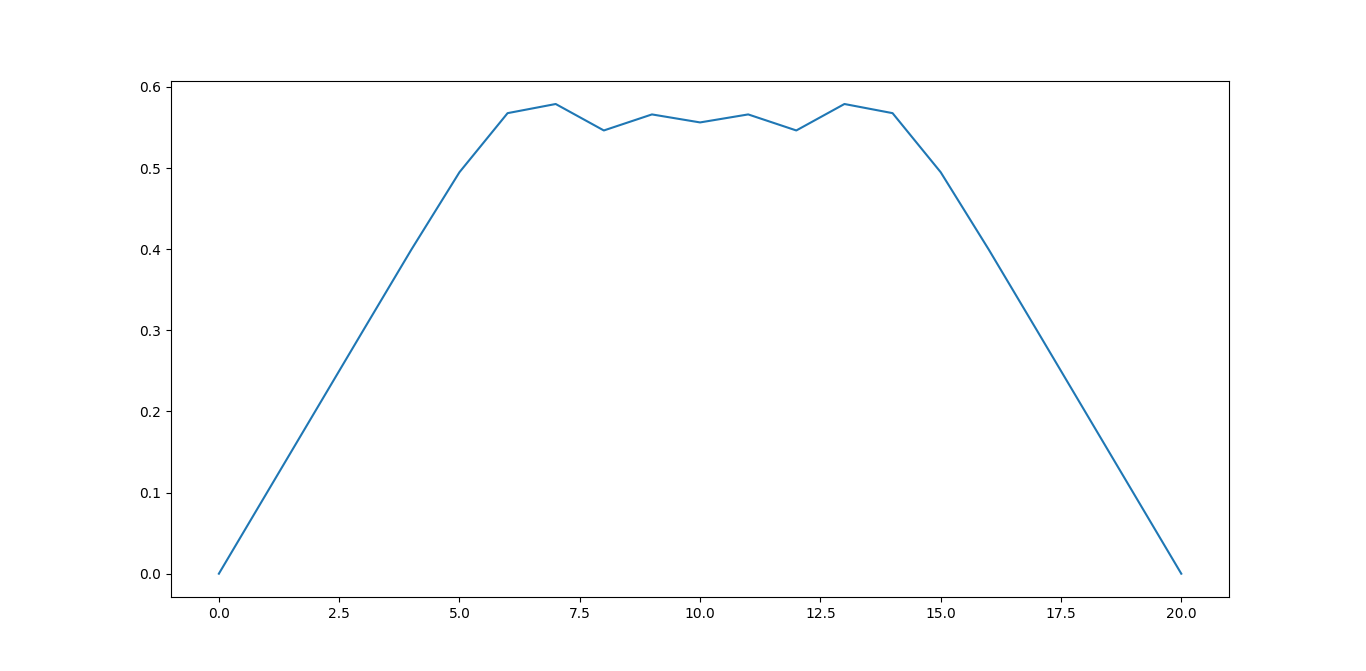
\includegraphics[width=0.5\textwidth]{des 1.png}
    \caption{Linea inicial}
\end{figure}
\begin{figure}[H]
    \centering
    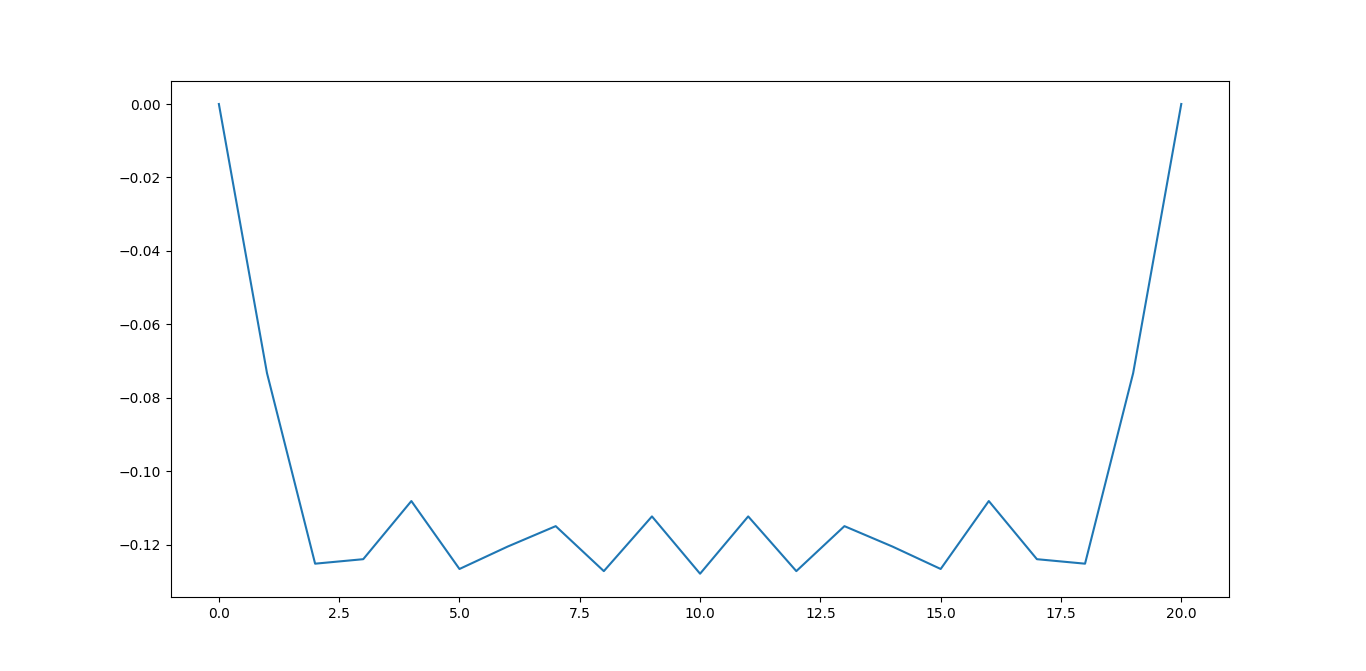
\includegraphics[width=0.5\textwidth]{des 3.png}
    \caption{Linea deformada}
\end{figure}
\section{Animación}
Para la animación usamos el modulo de Matplotlib ''FuncAnimation'', lo que haremos sera graficar una función de dos dimensiones en cada iteración. Esto se hará con cada columna de nuestra matriz U, obtenida luego de ejecutar nuestra funciones principal de la ecuación de onda.
\begin{lstlisting}[language=Python,caption=Animación]
def animar(i):
    plt.gca().clear()
    plt.gca().plot(np.arange(0,len(U[:,i])),U[:,i])
ani =animation.FuncAnimation(plt.gcf(),animar,range(0,U.shape[1]),interval=10,repeat_delay =1000)
\end{lstlisting}
\section{Conclusión}
\begin{itemize}
    \item Podemos encontrar la ecuación de onda en diversas situaciones,es por esto que es importante estudiar su comportamiento en distintas condiciones.
    \item Se pudo identificar la importancia de cumplir la condición de estabilidad, ya que una ligera alteración y el gráfico resultante se descontrola totalmente, obteniendo resultados que incluso no se pueden graficar correctamente.
    \item A pesar de tener muchas deformaciones e iteraciones en las que la función se vuelve muy irregular, la ecuación de onda llega a su mismo punto de inicio y repite este ciclo infinitamente.
    \item Se puede notar que las deformaciones en la ecuaciones siempre son simétricas, sin importar que tan irregular como en el caso de la función que tenia una forma triangular.
\end{itemize}
\section{Código completo}
https://github.com/ZzzandyzzZ/Fisica-Computacional
\end{document}


